\PassOptionsToPackage{table}{xcolor}
\documentclass[12pt,letterpaper,twocolumn,openany,nodeprecatedcode,bg=none]{dndbook}
\usepackage[english]{babel}
\usepackage[utf8]{inputenc}
\usepackage{longtable,booktabs,array}
\usepackage{calc}
\usepackage{etoolbox}
\usepackage{caption}
\usepackage{float}
\usepackage{graphicx}
\usepackage{needspace}
\usepackage{tikz}

% Reset zebra striping at the start of every table
\AtBeginEnvironment{longtable}{\rowcolors{1}{white}{gray!10}\small}
\AtBeginEnvironment{table}{\rowcolors{1}{white}{gray!10}}

\providecommand{\pandocbounded}[1]{#1}
\providecommand{\tightlist}{%
  \setlength{\itemsep}{0pt}\setlength{\parskip}{0pt}}

\captionsetup{labelformat=empty}
\setcounter{secnumdepth}{0}
\setlength{\parindent}{0pt}
\setlength{\parskip}{0.5\baselineskip}
\setlength{\headheight}{15pt}

% Prevent orphaned subsections
\let\oldsubsection\subsection
\renewcommand{\subsection}[1]{%
  \needspace{5\baselineskip}%
  \oldsubsection{#1}%
}

\begin{document}
\onecolumn

      \title{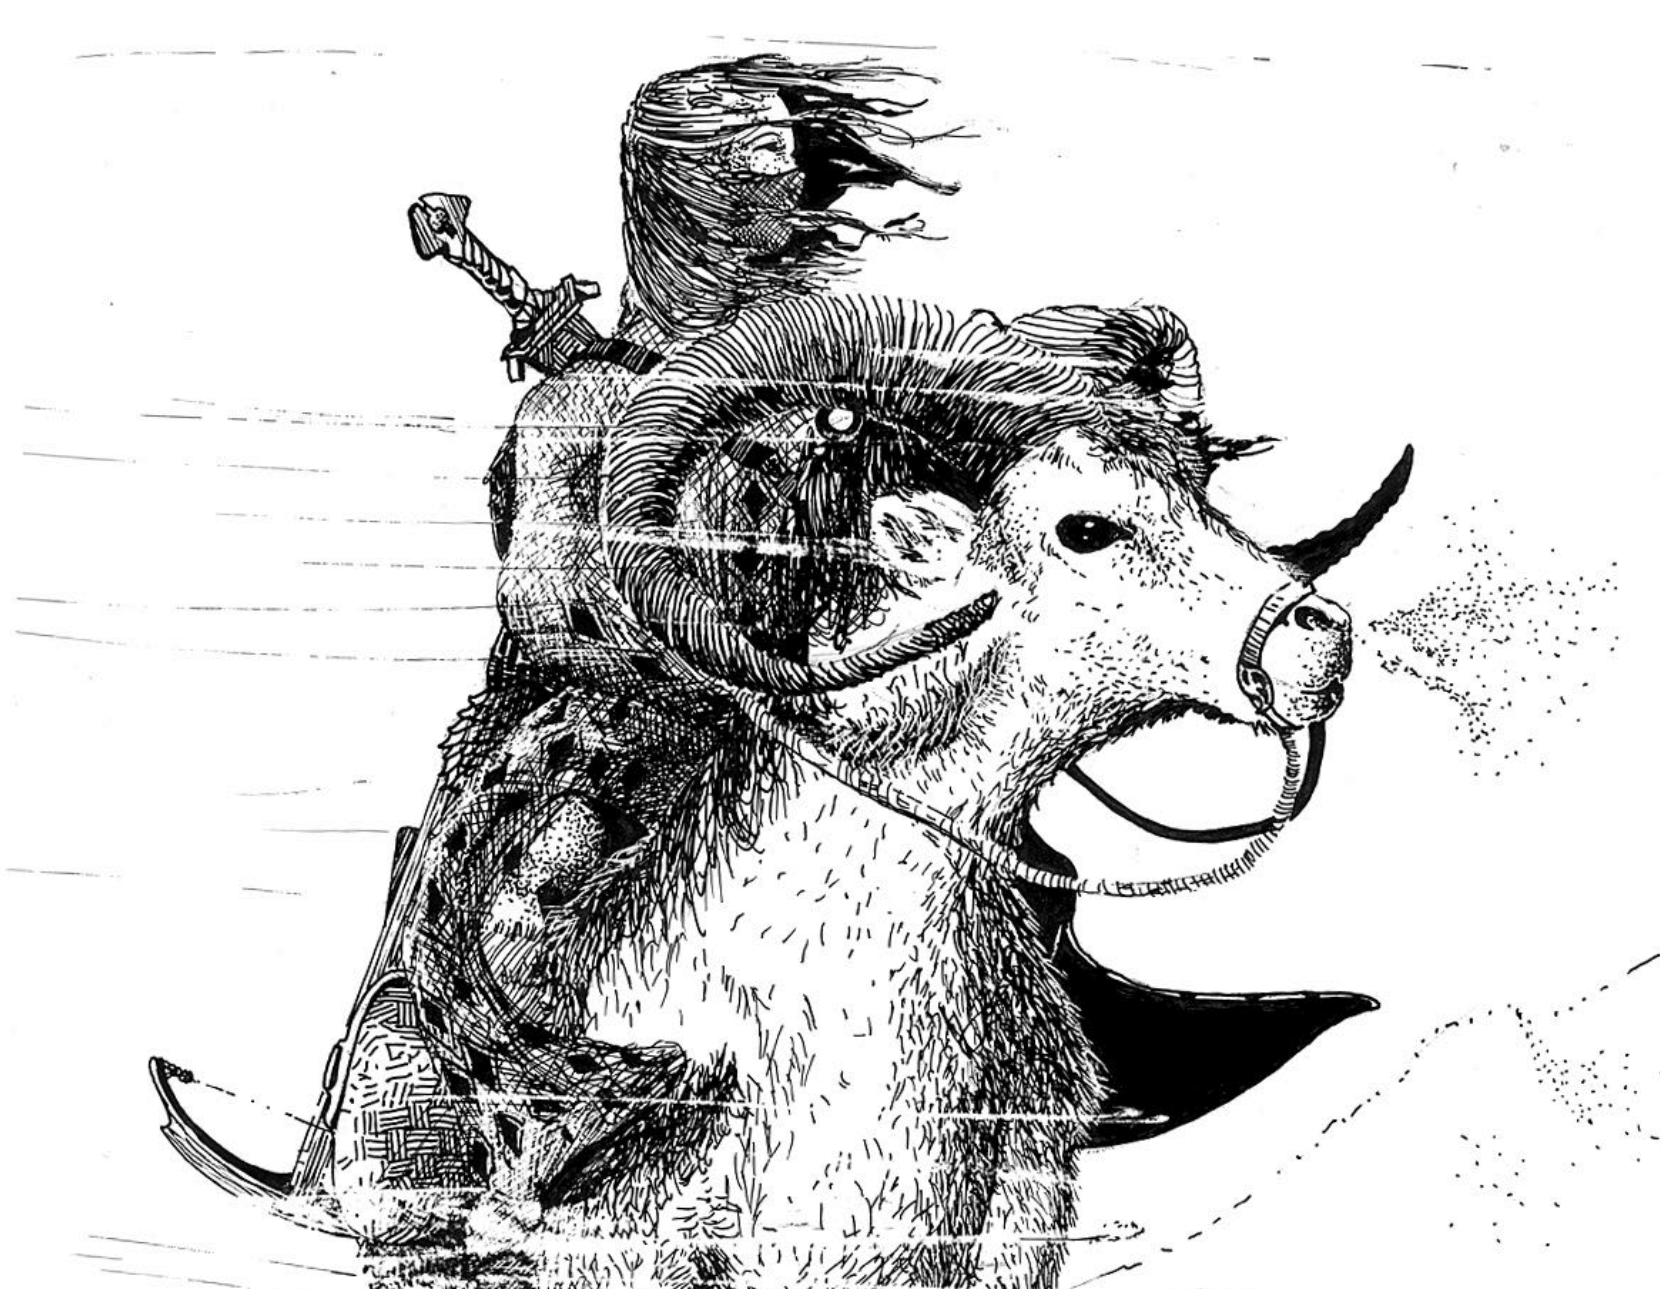
\includegraphics[width=0.9\textwidth,height=0.55\textheight,keepaspectratio]{wanderer.png}\\[1.5cm]Ranger}
  \author{Class Handbook}
\date{}
\maketitle

\clearpage
\thispagestyle{empty}
\null\vfill
\begin{center}{\Large\itshape Your trusty class handbook for fantasy
gaming.}\end{center}
\vfill


\clearpage
\twocolumn

\section{Ranger}\label{ranger}

\subsection{Core Ranger Traits}\label{core-ranger-traits}

\needspace{11\baselineskip}

{\def\LTcaptype{none} % do not increment counter
\begin{table}[!htbp]
\centering
\begin{tabular}{@{}
  >{\raggedright\arraybackslash}p{(\linewidth - 2\tabcolsep) * \real{0.3421}}
  >{\raggedright\arraybackslash}p{(\linewidth - 2\tabcolsep) * \real{0.6579}}@{}}
\toprule\noalign{}
\begin{minipage}[b]{\linewidth}\raggedright
\textbf{Primary Ability}
\end{minipage} & \begin{minipage}[b]{\linewidth}\raggedright
Strength
\end{minipage} \\
\midrule\noalign{}
\textbf{Hit Points} & 1d6 \\
\textbf{Saving Throw Proficiencies} & Strength, Dexterity \\
\textbf{Skill Proficiencies} & Choose 3 skills \\
\textbf{Weapon Proficiencies} & Choose 3 categories \\
\textbf{Starting Equipment} & Breastplate, Cloak, 2 Handaxes, 2 Daggers,
Longbow \\
\bottomrule\noalign{}
\end{tabular}
\end{table}
}

\subsection{Ranger Features}\label{ranger-features}

\needspace{20\baselineskip}

{\def\LTcaptype{none} % do not increment counter
\begin{table}[!htbp]
\centering
\begin{tabular}{@{}
  >{\raggedright\arraybackslash}p{(\linewidth - 4\tabcolsep) * \real{0.1087}}
  >{\raggedright\arraybackslash}p{(\linewidth - 4\tabcolsep) * \real{0.2391}}
  >{\raggedright\arraybackslash}p{(\linewidth - 4\tabcolsep) * \real{0.6522}}@{}}
\toprule\noalign{}
\begin{minipage}[b]{\linewidth}\raggedright
Level
\end{minipage} & \begin{minipage}[b]{\linewidth}\raggedright
Proficiency
\end{minipage} & \begin{minipage}[b]{\linewidth}\raggedright
Class Features
\end{minipage} \\
\midrule\noalign{}
1 & +2 & Rapid Strike, Natural Leader \\
2 & +2 & --- \\
3 & +2 & Superior Strike, Ability Bonus \\
4 & +2 & --- \\
5 & +2 & Whirling Strikes \\
6 & +2 & --- \\
7 & +2 & Ability Bonus \\
8 & +2 & --- \\
9 & +3 & Mighty Strikes \\
10 & +3 & --- \\
\bottomrule\noalign{}
\end{tabular}
\end{table}
}

\subsection{Level 1: Rapid Strike}\label{level-1-rapid-strike}

You can sacrifice power for rapid strikes.

\textbf{Swift Slash.} You can make two melee attacks as an action if you
wield two light weapons or a single non-light weapon, but you do not add
your ability modifier to your damage roll.

\textbf{Quick Shot.} You can make two ranged attacks as an action, but
you do not add your ability modifier to your damage roll.

\subsection{Level 1: Natural Leader}\label{level-1-natural-leader}

You have unmatched experienced roaming the wilds and leading
expeditions.

\textbf{Lead by Example.} When you make a check, you can provide
guidance to your allies. Until your next turn, friendly creatures within
30 feet of you can use your result in place of rolling that same check.

\textbf{Druidic Novice.} You have picked up druidic magic allowing you
to speak with animals. You must perform a ritual that takes 1 minute in
order to activate this ability which then lasts for 1 hour.

\subsection{Level 3: Superior Strike}\label{level-3-superior-strike}

You can make a total of three attacks when you use rapid strike.

\subsection{Level 3: Ability Bonus}\label{level-3-ability-bonus}

You gain a +1 bonus to two different abilities of your choice.

\subsection{Level 5: Whirling Strikes}\label{level-5-whirling-strikes}

You can make a total of four attacks when you use rapid strike.

\subsection{Level 7: Ability Bonus}\label{level-7-ability-bonus}

You gain a +1 bonus to two different abilities of your choice.

\subsection{Level 9: Mighty Strikes}\label{level-9-mighty-strikes}

You can now add your ability modifier to damage rolls for attacks made
with your Rapid Strike feature.

\onecolumn

\clearpage
\thispagestyle{empty}
\begin{center}
\vspace*{\fill}
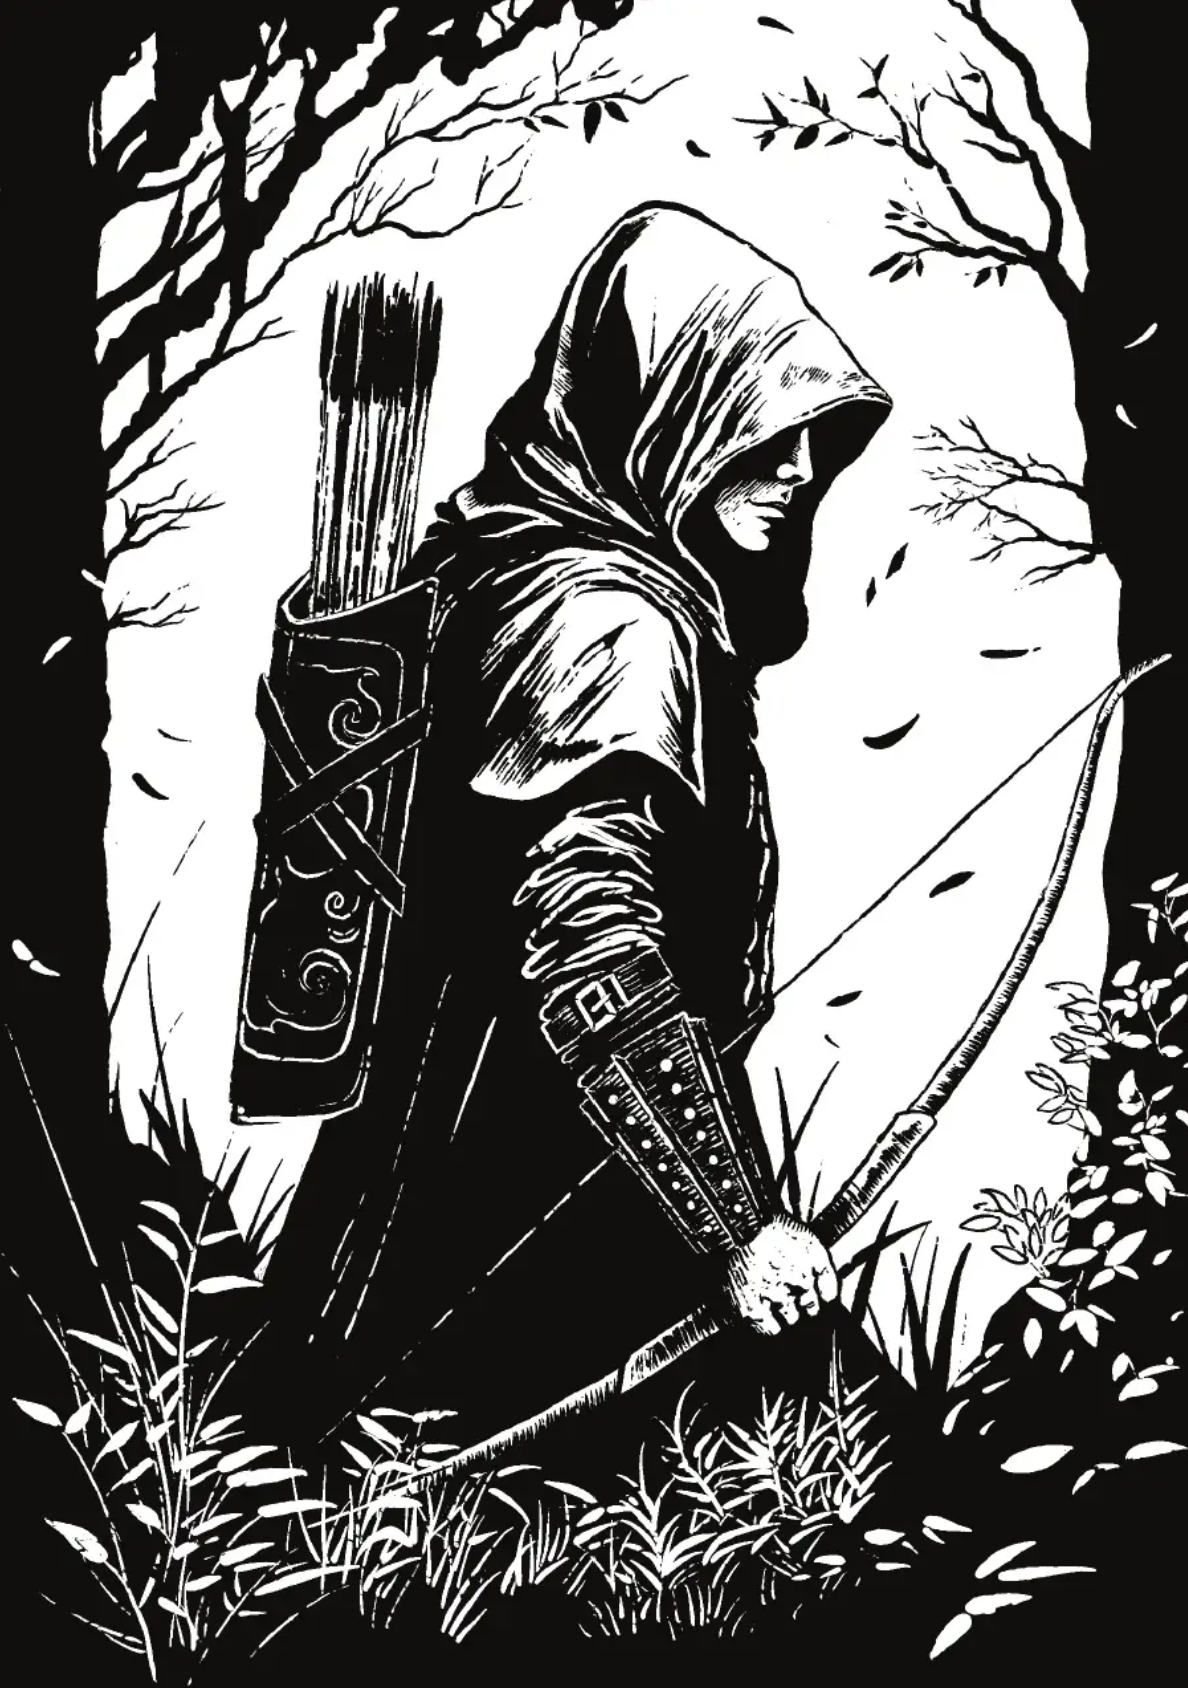
\includegraphics[width=0.7\textwidth,keepaspectratio]{rangerSD.png}\par
\vspace{0.4cm}
{\itshape A ranger is at home in the wilds}\par
\vspace*{\fill}
\end{center}

\end{document}